\chapter{Experiments}
The evolutionary algorithms described in section \ref{evolution-strategies} were implemented in C++. This language was chosen due to its flexibility, performance and the possibility to make use of the ngSPICE simulator. The implementation also utilizes the RInside \footnote{RInside home page - \url{http://dirk.eddelbuettel.com/code/rinside.html}} library which integrates R \footnote{R home page - \url{https://www.r-project.org/}} into C++ \cite{Rcpp}. The R language is used to plot graphs dynamically during the evolution either to the screen or to a file so the user can see and record how the solution evolves.

The program is written as a console application and the user can specify the properties of the evolution via command-line arguments. This approach also allows the user to easily run the application multiple times and collect the results of the evolution.

The results are in the form of graphs and a text output which contains the details about the evolution run. The graphs can be either dynamically generated to the screen during the program run or saved as files to the local drive as well as the text output. The user can specify how often the graphs and text description are generated, for example, each time the fitness function of the best chromosome in the population decreases by 1\%.

The results of the experiments discussed below are related to the evolutionary algorithm itself. The results of the optimization of the amplifiers are analyzed in sections \ref{single-stage-results} and \ref{2stage-results}.

\section{Initial stages of experiments}
The first experiments were performed only in order to optimize the value of resistor $R1$ in the single stage amplifier. The 'best match' evaluation method and mutations with one step size were used. The evolution always found a value close to \SI{50}{\kilo\ohm} which was the desired solution. These experiments were always successful as this was a very simple task for the evolution.

In the next stage, the task was to optimize the voltage divider constituted by $R1$ and $R2$. The 'best match' method and mutations with one step size were used again and it emerged, that the evolution was able to find the solution even faster than in the previous case. This was because we were looking only for the right ratio between the resistors and not for specific values so the set of the desired solutions was much larger in this case even though the search space was larger as well as it was two-dimensional.

The next task for the evolution was to find the right values for resistors $R1$, $R2$ and $Rg$. The evolution parameters were set in the same way as in the previous experiments. This task showed the weak spot of mutations with one step size as the evolution was able to find an acceptable solution very rarely. The reason was that the desired value of $Rg$ is very close to the lower bound of the search space (the analytical value is only \SI{40}{\ohm}). Since mutations with one step size use the same mutation value in every dimension, it was not possible to mutate $Rg$ only by a few ohms (not to move away from the lower bound of this dimension) and at the same time look for the right values in other dimensions which required steps in kiloohms. The value of $Rg$ heavily influences the overall fitness of the chromosome because high values significantly decrease the gain of the amplifier. The usual course of the evolution was that the value of $Rg$ converged quickly to the lower boundary and since this parameter has a great influence on the fitness, the evolution preferred chromosomes with this property. This led to a quick decrease of the mutation step size $\sigma$ (the fitness function also indirectly evaluates the value of $\sigma$) and the algorithm got stuck in a local optimum since other dimensions (values of other resistors) in the search space could not be searched properly. The solution to this problem was to implement mutations with $n$ step sizes discussed in section \ref{n-step}. This approach allows us to treat every dimension separately and therefore search the search space more effectively. After the implementation, the evolution was able to find a satisfactory solution in most of its runs.

The previous experiments proved that the evolutionary algorithms are able to provide acceptable solutions in the domain of analog amplifiers. The next section describes the process of determining the ideal parameters for the evolution.

\section{Evolution parameters}
In order to make the evolution strategies work efficiently, we need to find and set the correct parameters for the evolution.

The size of the search space is defined by the number of dimensions and by the size of every dimension. The number of dimensions depends on the number of electronic components that we want to optimize and the sizes of the dimensions depend on the range of the values that every component can have. These ranges were set from \SIrange{0}{200}{\kilo\ohm} for resistors and from \SIrange{0}{500}{\micro\farad} for capacitors. The upper bounds are based on the values of real electronic components so, for example, we do not expect to have a higher resistance than \SI{200}{\kilo\ohm} in the circuit. The values of some particular components could have a smaller range, for example, resistor $Rg$ which value does not need to be higher than a few kiloohms, but the assumption is that we have no knowledge about the circuit at all.

The initial mutation step size $\sigma$ is set to 100. This value is not very important because this parameter is adapted during the evolution. Experiments showed that there is no difference between setting the initial $\sigma$ to 10 or 500 for example. However, if we set the initial value too high (10000 and above), it is more likely that the evolution will get stuck in a local optimum because the algorithm converges too quickly at the start.

The experiments also showed that the values of the learning parameters $\tau$ and $\tau'$ have a significant impact on the speed at which the evolution converges to the optimum. The higher the values were, the faster the evolution converged, nevertheless this also means that the probability of finding only a local optimum was rapidly increased. For this reason, the values were set according to formulas \ref{set-tau} and \ref{set-tau-prime} to their lowest possible values. The parameter $n$ is the number of dimensions of the search space.

\begin{equation} \label{set-tau}
    \tau = \frac{1}{\sqrt{n}}
\end{equation}

\begin{equation} \label{set-tau-prime}
    \tau' = \frac{1}{\sqrt{2\sqrt{n}}}
\end{equation}

The maximum difference between the peak and trough of the amplifier's output waveform was empirically set to 25. This means that the values of the peak and trough of the waveform can differ at most by 25\%.

\section{Population size, selection type and selective pressure}
\label{population-size}
Important parameters of the evolution are numbers $\mu$ and $\lambda$ which define the population size (the number of parents and children in every generation) and the selective pressure which is defined by the ratio between $\mu$ and $\lambda$. The next important parameter is the type of the selection that we choose for the evolution (($\mu$, $\lambda$)-ES or ($\mu + \lambda$)-ES). In order to determine the most suitable values of the parameters, there were various experiments carried out which are summarized in table \ref{experiments-results}.

Every row of the table contains results for a different combination of $\mu$ and $\lambda$. The values of $\mu$ are set to 1, 5, 10 and 15 and the selective pressure is also 1, 5, 10 and 15 for every value of $\mu$, so there are four different values of $\lambda$ for every $\mu$. For every such combination, there are results for both selection types and under every type, there are three columns representing all the three evaluation methods that are discussed in chapter \ref{chromosomes-evaluation}. One cell of the table corresponds to the result of one experiment where the evolutionary algorithm was run 10 times with the same parameters and the fitness values of the resulting chromosomes were added up and divided by 10. The task was to optimize the single stage amplifier.

We can see that there is no significant difference between the selection schemes, provided the selective pressure is higher than one. On lines 5, 9 and 13 (where the selection pressure is 1) the ($\mu$, $\lambda$)-ES scheme performs significantly worse than the ($\mu + \lambda$)-ES scheme and even increasing the population size has no effect (line 5 compared to line 9 and 13). However, when we sum up all the values in both schemes (excluding lines 1, 5, 9 and 13), the latter one gives us better results, so the ($\mu + \lambda$)-ES selection scheme was chosen as the more effective one.

We can also see that when the value of $\mu$ is only 1, the algorithm's results are substantially worse than in the rest of the table and on the other hand when we increase it from 5 to 15, there is only a small change in the overall performance.

The value of $\lambda$ is set according to the value of $\mu$ multiplied by the selection pressure and it highly influences the overall computation time of the algorithm because it defines the number of chromosomes that have to be evaluated in every generation (the evaluation includes the amplifier's simulation which takes most of the computation time). When the selective pressure and the value of $\mu$ are higher than one, the overall efficiency of the algorithm does not increase rapidly but there is a noticeable increase in the computation time. For this reason, the values of $\mu$ and $\lambda$ were set to $\mu = 15$ and $\lambda = 150$ as a compromise between the algorithm's time demands and the optimization efficiency. Higher values were also examined but they did not provide any significant improvements.

\begin{table}[H]
\centering
\begin{tabular}{@{}ccccccccc@{}}
\toprule
    &       &           & \multicolumn{3}{c}{($\mu$, $\lambda$)-ES} & \multicolumn{3}{c}{($\mu + \lambda$)-ES} \\
   \cmidrule(lr){4-6} \cmidrule(lr){7-9}
    & $\mu$ & $\lambda$ & best match & ideal sin & max. ampl.       & best match & ideal sin  & max. ampl.     \\
   \midrule
1.  & 1     & 1         & N/A        & N/A       & N/A              & 21.82      & 99.00      & 2.90           \\
2.  & 1     & 5         & 20.82      & 113.75    & 1.98             & 13.44      & 57.91      & 2.69           \\
3.  & 1     & 10        & 18.84      & 76.81     & 1.40             & 24.70      & 75.01      & 2.84           \\
4.  & 1     & 15        & 18.43      & 128.75    & 2.26             & 19.52      & 34.11      & 1.02           \\
5.  & 5     & 5         & 49.62      & 169.02    & 36.50            & 9.81       & 56.61      & 3.18           \\
6.  & 5     & 25        & 7.28       & 55.00     & 3.12             & 12.12      & 34.88      & 2.72           \\
7.  & 5     & 50        & 16.18      & 64.22     & 3.21             & 9.75       & 43.73      & 3.57           \\
8.  & 5     & 75        & 3.70       & 58.82     & 3.10             & 4.20       & 38.84      & 3.52           \\
9.  & 10    & 10        & 49.41      & 154.66    & 26.40            & 8.94       & 53.77      & 3.18           \\
10. & 10    & 50        & 9.09       & 60.93     & 2.68             & 7.02       & 45.04      & 3.58           \\
11. & 10    & 100       & 6.97       & 38.02     & 3.16             & 4.91       & 26.06      & 3.10           \\
12. & 10    & 150       & 8.06       & 25.54     & 3.10             & 2.52       & 23.07      & 3.07           \\
13. & 15    & 15        & 44.48      & 165.76    & 34.99            & 2.54       & 47.69      & 3.18           \\
14. & 15    & 75        & 4.64       & 56.18     & 2.25             & 4.96       & 51.74      & 3.56           \\
15. & 15    & 150       & 6.63       & 47.32     & 3.52             & 6.36       & 12.19      & 1.60           \\
16. & 15    & 225       & 7.56       & 31.17     & 2.65             & 0.70       & 19.31      & 1.08           \\
    \bottomrule
\end{tabular}
\caption{Results of experiments, cells contain results where the evolution was run 10 times and the fitness values of the resulting chromosomes were added up and divided by 10}
\label{experiments-results}
\end{table}


All the evolution parameters discussed above are summarized in table \ref{evolution-parameters}. These parameters were chosen as the most appropriate ones.

\begin{table}[H]
\centering
\begin{tabular}{@{}ll@{}}
\toprule
    Parameter                   & Value \\ \midrule
    Resistance range            & \SIrange{0}{200}{\kilo\ohm} \\
    Capacitance range           & \SIrange{0}{500}{\micro\farad} \\
    initial $\sigma$            & 100 \\
    max. peak-trough difference & 25 \% \\
    $\mu$                       & 15 \\
    $\lambda$                   & 150 \\
    selection type              & ($\mu + \lambda$)-ES \\
    $\tau$                      & equation \ref{set-tau}\\
    $\tau'$                     & equation \ref{set-tau-prime} \\ \bottomrule
\end{tabular}
\caption{Optimal evolution parameters}
\label{evolution-parameters}
\end{table}

\section{The typical course of the evolution}
Figure \ref{evolution-course} shows the typical course of the evolution. The population size parameters were set to $\mu = 10$ and $\lambda = 100$ and the terminating condition of the algorithm was that the evolution ends when the value of the fitness function of the best chromosome does not decrease by more than 1\% after 300 generations.

The green line represents the fitness of the best chromosome (the one with the lowest fitness) in every generation, the blue line is the fitness of the worst chromosome and the red line is the average fitness of every generation. In this case, we pick the chromosomes only from the set of $\mu$ parents. We can see that the red line is very close to the green line so the average fitness of every generation is close to the fitness of the best chromosome and that the blue line is scattered above the other two lines.

The evolution was stuck in a local optimum for approximately 20 generations between the 80th and 100th generation and the solution was evolved approximately after 300 generations. When the blue line is close the other two lines, it means that the sizes of the mutation steps $\sigma$ are low and the algorithm searches only a small area of the search space. When the values of $\sigma$ are low (close to zero), we can stop the algorithm after a few hundreds of generations because it will not provide any better solution than the current one and the resulting fitness is either in a local or global optimum.

The amount of generations needed for the optimization is usually a few hundred, as also shown in figure \ref{evolution-course}. When the size of the population is low (for example $\mu = 1$ and $\lambda = 5$), the optimization takes a few thousands of generations. In any case, there is approximately up to 30000 simulations in every evolution run which takes a few minutes (usually between two to four minutes) on the Intel Core i5-5200U processor.

In this case, the evaluation method was the 'best match' method and this evolution run was successful since the resulting fitness was very close to zero. With this method, we can consider those solutions which fitness is under 0.5 as sufficient because the amplifier's output waveform is very close to the desired one. The resulting value of the fitness of the best chromosome was 0.19.

\begin{figure}[H]
    \centerline{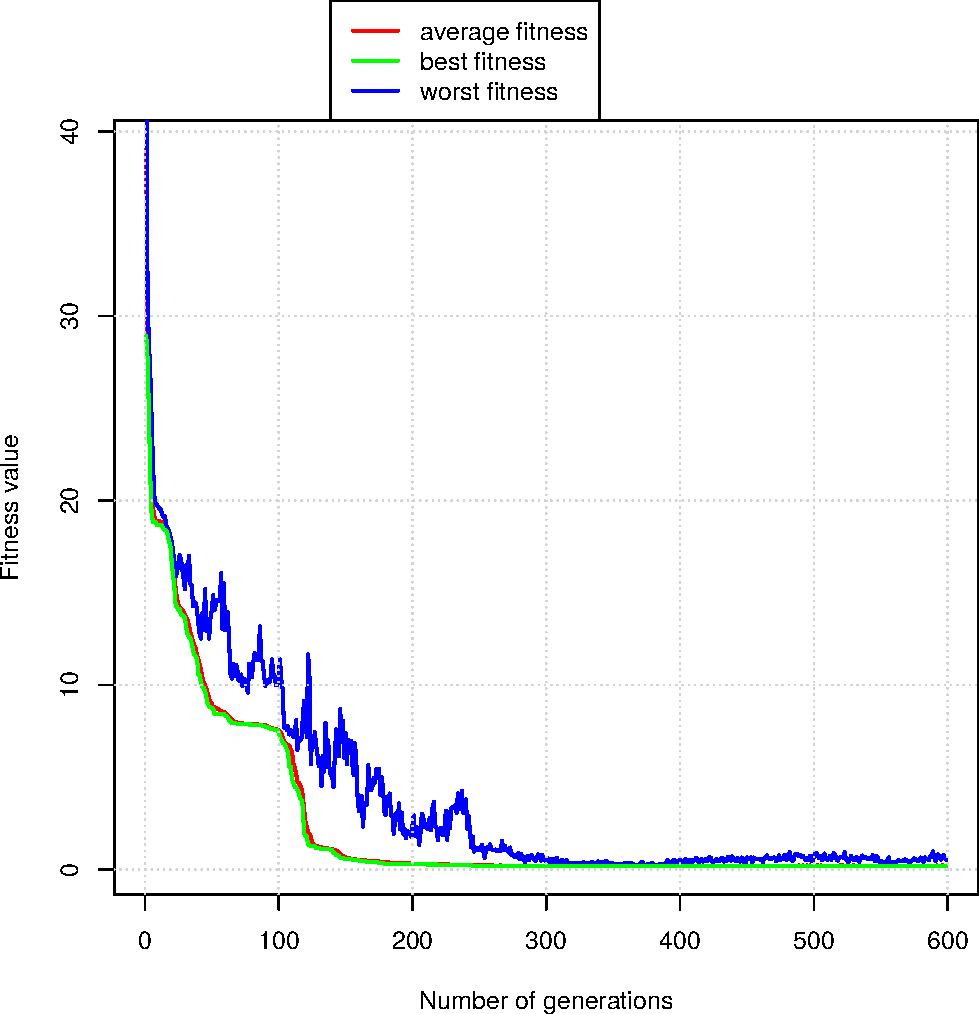
\includegraphics[scale=0.6]{evolution-course}
    \label{evolution-course}}
    \caption{The typical course of the evolution}
\end{figure}

\section{Single stage amplifier optimization} \label{single-stage-results}
Every evaluation method implemented in this thesis provides different means by which we can optimize the circuit.

The 'best match' method can be used for finding such properties that provide us the most similar output compared to the analytical solution. We optimize the values of 8 electronic components and experiments with this method proved that there are many other possible combinations which provide almost identical behaviour of the amplifier. Five examples are shown in table \ref{best-fit-solutions}. The simulation output of the amplifier with these values of components was visually identical with the analytical solution.


\begin{table}[H]
\centering
\begin{tabular}{@{}c ccccccc@{}}
\toprule
    $R1$ [\si{\kilo\ohm}] & $R2$ [\si{\kilo\ohm}] & $Re$ [\si{\ohm}] & $Rg$ [\si{\ohm}] & $Rc$ [\si{\kilo\ohm}] & $Ce$ [\si{\nano\farad}] & $Cin$ [\si{\nano\farad}] & $Cout$ [\si{\nano\farad}] \\
    \midrule
    200   & 76.2 & 7510  & 471 & 21.7 & 460     & 29    & 1010 \\
    78.5  & 16   & 3370  & 429 & 23   & 228 000 & 17    & 396 000 \\
    141   & 11.5 & 180   & 483 & 21.1 & 285 000 & 21    & 280 000 \\
    82.3  & 44.3 & 8590  & 400 & 16   & 499     & 202   & 95 \\
    118   & 41.2 & 11500 & 559 & 35.4 & 419     & 95    & 19 \\
    \bottomrule
\end{tabular}
\caption{Values of components that provide visually identical outputs with the analytical solution}
\label{best-fit-solutions}
\end{table}

The 'maximal amplitude' method can be used for finding the best amplification capabilities of the circuit as it does not take into consideration the shape of the output signal. This method is useful for the 'ideal sine' method because it allows us to find the appropriate maximal amplitude and then we can find the right waveform by using the latter method. By this approach, we can find even better solutions than the analytical one. One of such solutions is shown in figure \ref{better-solution-fig} and the values of the components are summarized in table \ref{better-solution-tab}. Since the amplitude of the input signal was $Vin = \SI{100}{\milli\volt}$ and the amplitude of the output signal is approximately \SI{4.2}{\volt}, the gain of this amplifier is approximately 42 (the gain of the analytically solved amplifier is approximately 18). The gain also depends on the voltage $V1$ that supplies the amplifier which is set to $V1 = \SI{12}{\volt}$ in the experiments.

\begin{figure}[!htb]
    \centerline{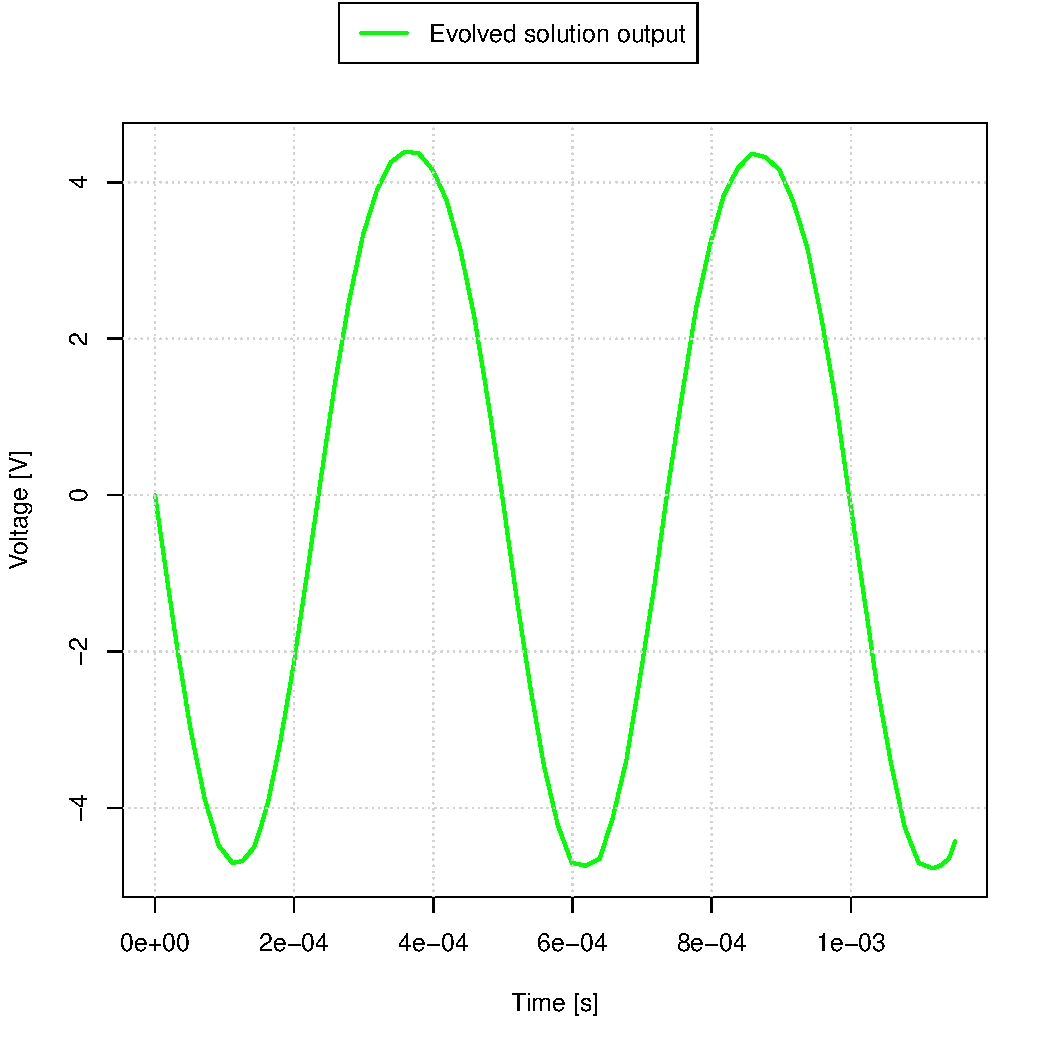
\includegraphics[scale=0.6]{best-solution-single-stage}\label{better-solution-fig}}
    \caption{The best solution for the single stage amplifier found by the evolution}
\end{figure}

\begin{table}[H]
\centering
\begin{tabular}{@{}cccccccc@{}}
\toprule
    $R1$ [\si{\kilo\ohm}] & $R2$ [\si{\kilo\ohm}] & $Re$ [\si{\ohm}] & $Rg$ [\si{\ohm}] & $Rc$ [\si{\kilo\ohm}] & $Ce$ [\si{\micro\farad}] & $Cin$ [\si{\micro\farad}] & $Cout$ [\si{\nano\farad}] \\
    \midrule
    168 & 15.1 & 169 & 49 & 4.21 & 16 & 274 & 86 \\
    \bottomrule
\end{tabular}
\caption{The best solution for the single stage amplifier found by the evolution}
\label{better-solution-tab}
\end{table}

The 'ideal sine' evaluation method also provides a universal tool for finding the appropriate values of components which produce an arbitrary amplification of the amplifier up to the maximal amplitude.

\section{Two stage amplifier optimization} \label{2stage-results}
This amplifier was chosen as the more complicated task to optimize. There was no analytical solution for this circuit so it was not possible to use the 'best match' evaluation method. Experimenting with this type of amplifier showed that this amplifier is much more difficult to optimize and that it does not provide any better amplification properties than the previous single stage amplifier.

The same set of experiments was carried out as for the previous amplifier and one of the best solutions is shown in figure \ref{best-solution-two-stage-fig}.

\begin{figure}[ht]
    \centerline{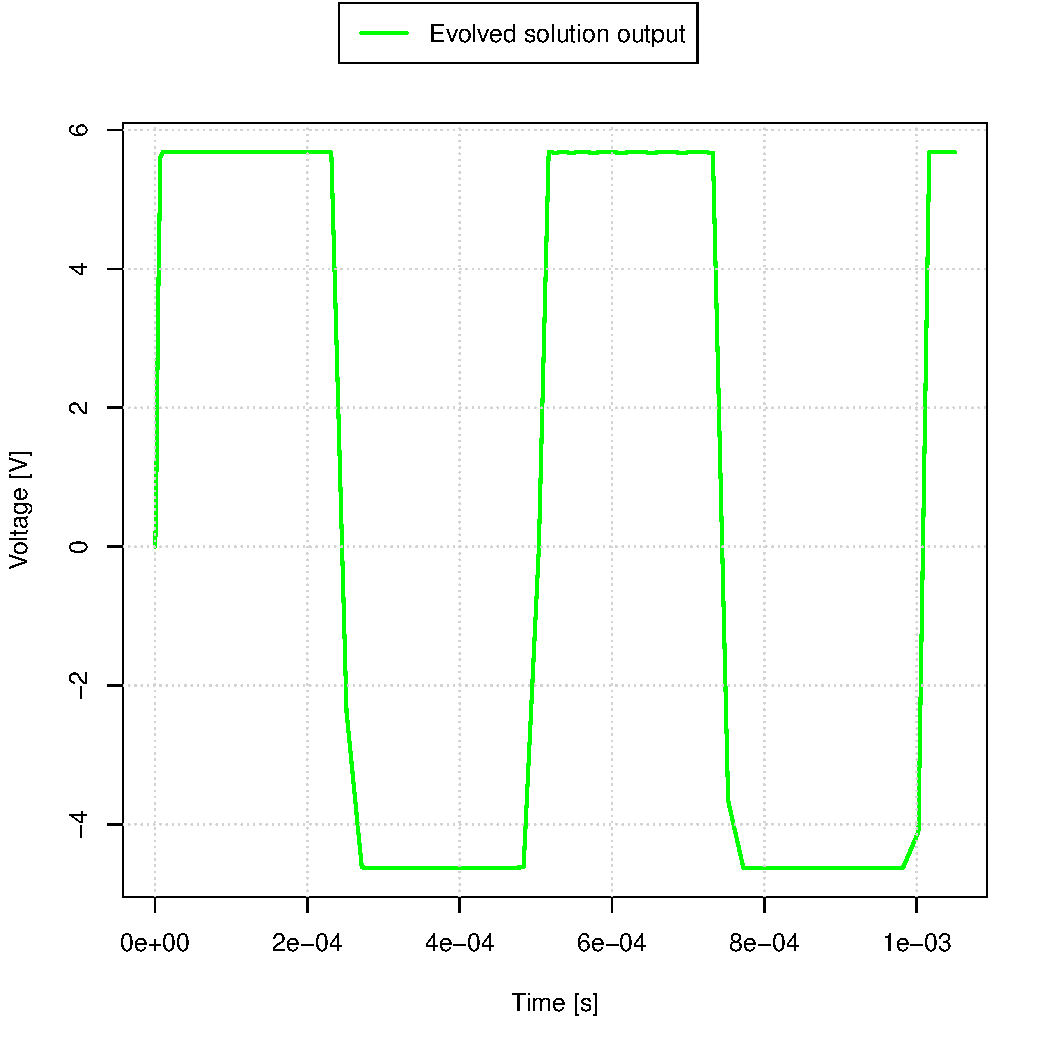
\includegraphics[scale=0.6]{best-solution-two-stage}\label{best-solution-two-stage-fig}}
    \caption{The best solution for the two stage amplifier found by the evolution}
\end{figure}

We can see that the resulting gain is approximately 50 (the amplitude of the input voltage is $Vin = \SI{100}{\milli\volt}$, the amplitude of the output voltage is approximately \SI{5}{\volt}, the supply voltage is $V1 = \SI{12}{\volt}$) but the output waveform is significantly distorted --- the circuit generates a square wave. The experiments did not provide any solution that would generate a sine wave. The components values for this solution are stated in table \ref{best-solution-two-stage-tab}.

\begin{table}[H]
\centering
\begin{tabular}{@{}cccccccccccccc@{}}
\toprule
    $R1$ [\si{\kilo\ohm}] & $R2$ [\si{\kilo\ohm}] & $Re$ [\si{\kilo\ohm}] & $Rc$ [\si{\kilo\ohm}] & $Ce$ [\si{\micro\farad}] & $Cin$ [\si{\micro\farad}] & $Cout$ [\si{\micro\farad}] \\
    $Rgb$ [\si{\ohm}] & $Reb$ [\si{\ohm}] & $Rcb$ [\si{\kilo\ohm}] & $R2b$ [\si{\kilo\ohm}] & $R1b$ [\si{\kilo\ohm}] & $Cm$ [\si{\micro\farad}] & $Ce2$ [\si{\micro\farad}] \\
    \midrule
    114 & 57  & 51.6 & 81.7 & 98   & 215 & 479 & \\
    22  & 298 & 3.37 & 9.24 & 80.5 & 351 & 139   \\
    \bottomrule
\end{tabular}
\caption{The best solution for the two stage amplifier found by the evolution}
\label{best-solution-two-stage-tab}
\end{table}